\newpage
\section{Задание 8.}

Найти поток векторного поля $\vv{a}(x, y, z)$ через замкнутую поверхность S (нормаль внешняя). Вычислить двумя способами: с помощью поверхностного и тройного интеграла.

 $$\vv{a} =3xz\vv{i} - 2x\vv{j}+y\vv{k},\quad S: x+y+z = 2, x=1, x=0, y =0, z =0$$

\subsection{Решение с помощью тройного интеграла.}

Воспользуемся теоремой Остроградского-Гаусса.

$$\Pi_S(\vv{a}) = \iint \limits_S \vv{a} \cdot \vv{N_0} \, dS = \iiint \limits_V (\text{div}\vv{a})\,dV$$

Посчитаем дивергенцию векторного поля $\vv{a}$.
$$\text{div}\vv{a} = \nabla \cdot \vv{a} = \dfrac{\partial}{\partial x}\left(3xz\right) + \dfrac{\partial}{\partial y}\left(- 2x\right) + \dfrac{\partial}{\partial z}\left(y\right) = 3z + 0 + 0 = 3z$$
\begin{center}
    
Теперь подставим.

$$\iiint \limits_V (\text{div}\vv{a})\,dV = \iiint \limits_V 3z \,dV$$

Теперь определимся с границами интегрирования. $x\in[0,1]$, $y\in[0,\leq 2-x]$, $z\in[0,2-x-y]$

$$\iiint \limits_V 3z \,dV = \int_0^1 \, dx \int_{0}^{2-x}\,dy \int_{0}^{2-x-y} 3z\, dz$$

Интегрируем по $z$.
$$ \int_{0}^{2-x-y} 3z \, dz = 3\left[ \frac{z^2}{2} \right]_{0}^{2-x-y} = \frac{3(2-x-y)^2}{2} $$
Интегрируем по $y$.
$$ \int_{0}^{2-x} \frac{3(2-x-y)^2}{2} \, dy = \frac{3}{2} \int_{0}^{2-x} (4 - 4x - 4y + x^2 + 2xy + y^2) \, dy = \frac{3}{2} \left[ 4y - 4xy - 2y^2 + x^2y + xy^2 + \frac{y^3}{3} \right]_{0}^{2-x} =$$
$$ =\frac{1}{2} \left[ 12y - 12xy - 6y^2 + 3x^2y + 3xy^2 + y^3\right]_{0}^{2-x} =$$ 
$$=\frac{1}{2} \left[ 12(2-x) - 12x(2-x) - 6(2-x)^2 + 3x^2(2-x) + 3x(2-x)^2 + (2-x)^3\right] = ... =$$ 
$$=\frac{1}{2}\left[-x^3 + 6x^2 - 12x + 8\right]$$
Интегрируем по $x$.
$$\frac{1}{2}\int_0^1 -x^3 + 6x^2 - 12x + 8\, dx = \frac{1}{2}\left[ \frac{x^4}{4} + 2x^3 - 6x^2 + 8x \right]_0^1 = \frac{1}{2}\left( -\frac{1^4}{4} + 2 \cdot 1^3 - 6 \cdot 1^2 + 8 \cdot 1 \right) =$$
$$=\frac{1}{2}\left(-\frac{1}{4} + 2 - 6 + 8\right) = \frac{1}{2}\cdot\frac{-1 + 8 - 24 + 32}{4} = \boxed{\frac{15}{8}}$$
\end{center}

\newpage
\subsection{Решение с помощью поверхностного интеграла.}

$$\Pi_S(\vv{a}) = \iint \limits_S \vv{a} \cdot \vv{N_0} d\vv{S}$$


\begin{figure}[h!t]
    \centering
    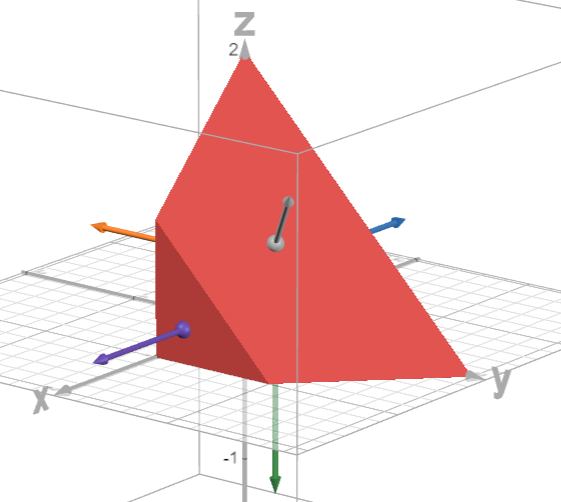
\includegraphics[width=0.75\linewidth]{Task8/Normal_vectors.png}
    \caption{Задание 8. Форма фигуры, с её векторами нормали.\underline{\href{https://www.desmos.com/3D/p0j1s5t0mn}{(Desmos)}}.}
\end{figure}
\begin{center}


Разделим интеграл на 5 поверхностей.

$$\iint \limits_S = \iint \limits_{\text{верхняя}} + \iint \limits_{\text{передняя}} + \iint \limits_{\text{левая}} + \iint \limits_{\text{задняя}} + \iint \limits_{\text{нижняя}}$$
Теперь перейдем к самой увлекательной части.

$$\iint \limits_{\text{верхняя}} \vv{a} \cdot \vv{N_0} d\vv{S} = \dfrac{1}{\sqrt{3}}\iint \limits_{\text{верхняя}} (3xz, - 2x, + y) \cdot (1,1,1))\, d\vv{S} = \dfrac{1}{\sqrt{3}}\iint \limits_{\text{верхняя}} 3xz - 2x + y\, d\vv{S}$$$$\begin{cases}
    z(x,y)=2-x-y\\
    d\vv{S} = \sqrt{1 + \left(\frac{\partial z}{\partial x}\right)^2 + \left(\frac{\partial z}{\partial y}\right)^2}\,dx\,dy
\end{cases} \Rightarrow \quad d\vv{S} = \sqrt{1 + (-1)^2 + (-1)^2}\,dx\,dy = \sqrt{3}\,dx\,dy$$
$$= \sqrt{3}\cdot\dfrac{1}{\sqrt{3}} \int_0^1\,dx \int_0^{2-x} 3x(2-x-y) - 2x + y\,dy = \int_0^1\,dx\int_{0}^{2-x} (4x - 3x^2 - 3xy + y) \, dy = $$
$$=\int_0^1\left[ (4x - 3x^2)y - \frac{3xy^2}{2} + \frac{y^2}{2} \right]_{0}^{2-x}\,dx =\int_0^1 (4x - 3x^2)(2 - x) - \frac{3x(2 - x)^2}{2} + \frac{(2 - x)^2}{2}\,dx =  $$
$$ \int_{0}^{1} \left( 2 + \frac{3x^3}{2} - \frac{7x^2}{2} \right) \, dx = \left[ 2x + \frac{3x^4}{8} - \frac{7x^3}{6} \right]_{0}^{1} = \left( 2 + \frac{3}{8} - \frac{7}{6} \right) = \left( 2 + \frac{9}{24} - \frac{28}{24} \right) =$$ 
$$= \left( 2 - \frac{19}{24} \right) = \left( \frac{48}{24} - \frac{19}{24} \right) = \frac{29}{24} $$

$$\iint \limits_{\text{передняя}} \vv{a} \cdot \vv{N_0}\, d\vv{S} = \iint \limits_{\text{передняя}} (3xz, - 2x, + y) \cdot (1,0,0))\, d\vv{S} =\iint \limits_{\text{передняя}} 3xz\, d\vv{S} = \int_0^1\,dy \int_0^{1-y} 3xz\,dz = $$
$$=\left\{\text{тут $x=const=1$}\right\} = 3\int_0^1\,dy \int_0^{1-y} z\,dz = \dfrac{3}{2}\int_0^1 (1-y)^2 \,dy = \dfrac{3}{2}\left[y - y^2 + \dfrac{y^3}{3}\right]_0^1 = \dfrac{3}{2}\left[1 - 1 + \dfrac{1}{3}\right] = \dfrac{1}{2}$$

$$\iint \limits_{\text{левая}} \vv{a} \cdot \vv{N_0}\, d\vv{S} = \iint \limits_{\text{левая}} (3xz, - 2x, + y) \cdot (0,-1,0))\, d\vv{S} = \iint \limits_{\text{левая}}2x\, d\vv{S} = \int_0^1\, dx \int_0^{2-x} 2x\,dz = $$ 
$$ = \int_0^1 2x(2-x) \, dx = 2\int_0^1 2x-x^2 \, dx = 2\left[x^2 - \dfrac{x^3}{3}\right]_0^1 = 2\left[1 - \dfrac{1}{3}\right] = \dfrac{4}{3}$$

$$\iint \limits_{\text{задняя}} \vv{a} \cdot \vv{N_0}\, d\vv{S} = \iint \limits_{\text{задняя}} (3xz, - 2x, + y) \cdot (-1,0,0))\, d\vv{S} = \iint \limits_{\text{задняя}} -3xz\, d\vv{S} = $$ 
$$ = \left\{\text{тут $x=0$ на всей поверхности}\right\} = 0$$ 

$$\iint \limits_{\text{нижняя}}\vv{a} \cdot \vv{N_0}\, d\vv{S} = \iint \limits_{\text{нижняя}} (3xz, - 2x, + y) \cdot (0,0,-1))\, d\vv{S} = \iint \limits_{\text{нижняя}} -y \,d\vv{S} = -\int_0^1\, dx \int_0^{2-x} y\,dy = $$
$$ = -\dfrac{1}{2}\int_0^1 (2-x)^2 \, dx = -\dfrac{1}{2}\int_0^1 4-4x+x^2 \, dx = -\dfrac{1}{2}\left[4x - 2x^2 + \dfrac{x^3}{3}\right]_0^1 = -\dfrac{1}{2}\left[4 - 2 + \dfrac{1}{3}\right] = -\dfrac{7}{6}$$

$$\iint \limits_S \vv{a} \cdot \vv{N_0} d\vv{S} = \frac{29}{24} + \frac{1}{2} + \dfrac{4}{3} + 0 - \dfrac{7}{6} = \boxed{\dfrac{15}{8}}$$

Ответы сошлись, мы победили :)

\end{center}
